\chapter{\textit{Projeto/Proposta de Solução}}
	\label{ch:proposta}

Os conceitos revisados até este momento seram utilizados para a criação de uma proposta de solução computacional para a equipe baja Velociraptor. Revisando, a equipe tem como principal problema não conseguir obter informações que interessam a cada setor do veículo de maneira \textbf{intuitiva, simplificada, modular e com armazenamento.} Estes três conceitos são detalhados na Tabela \ref{tab:cenario} a seguir:     

\begin{table}[!htb]
	\centering
		\caption{Conceitos do cenário estudado}
		\label{tab:cenario}
	\begin{tabular}{|l|l|l|}
		\hline
		\rowcolor[HTML]{9B9B9B} 
		{\color[HTML]{000000} Conceito} & {\color[HTML]{000000} Descrição}                                                                                                                                 \\ \hline
		Intuitiva                       & \begin{tabular}[c]{@{}l@{}}Demostração dos dados com \\ gráficos e valores absolutos\end{tabular}                                                                \\ \hline
		Simplificada                    & \begin{tabular}[c]{@{}l@{}}Um sistema para aquisição \\ para todos os dados dos sensores\\ reunindo as informações de \\ todos os setores do veículo\end{tabular} \\ \hline
		Modular                    & \begin{tabular}[c]{@{}l@{}}Preparado para expansão e\\  atualização com novas \\tecnologias\end{tabular} \\ \hline
		Armazenamento                   & \begin{tabular}[c]{@{}l@{}}Armazena os dados retirados \\ dos sensores para análises \\ futuras\end{tabular}                                                     \\ \hline
	\end{tabular}
\end{table}

\section{Objetivos}
\label{sec:objetivos}
Os objetivos que devem nortear o trabalho a fim de sanar os problemas levantados podem ser subdivididos em objetivo principal, que é a meta final do trabalho, e objetivos secundários, que servem para medir a acertividade das medidas tomadas no curso do trabalho.

\subsection{Objetivo Geral}

Produzir um sistema que forneça a equipe informações que irão ajudar aos setores do veículo (suspensão dianteira, suspensão traseira, freio, transmissão, eletrônica) em testes de bancada, bem como fornecer dados de uso geral da equipe como média do consumo de gasolina em prova para análises posteriores. 

O sistema é dividido em duas frentes: a parte de \textbf{aquisição} dos dados, feito junto ao SCOB com base nos dados recebidos via sensores revisados na seção \ref{sec:sensores}, esta parte já existe atualmente no baja Velociraptor, porém ela deve ser atualizada para acompanhar os avanços do novo \textit{software}; a parte de \textbf{tratamento} dos dados é o foco deste trabalho, nesta parte os dados serão armazenados de um cartão SD no SCOB e quando conectados a computadores de boxes, seus dados ali contidos são lidos por um \textit{software} que permite vizualição de gráficos e mostra de valores absolutos de maior importância. A Figura \ref{fig:geral} é um diagrama explicando o esquema geral do sistema, desde a aquisição dos dados pelos SCOBs e tratamento nos boxes com o \textit{software}. Os balões em azul indicam os sensores, os balões em laranja indicam \textit{hardware} e balões em verde indicam \textit{software}.         

\begin{figure}[!htb]
	\centering
		\caption{Diagrama com o esquema geral do sistema.}
		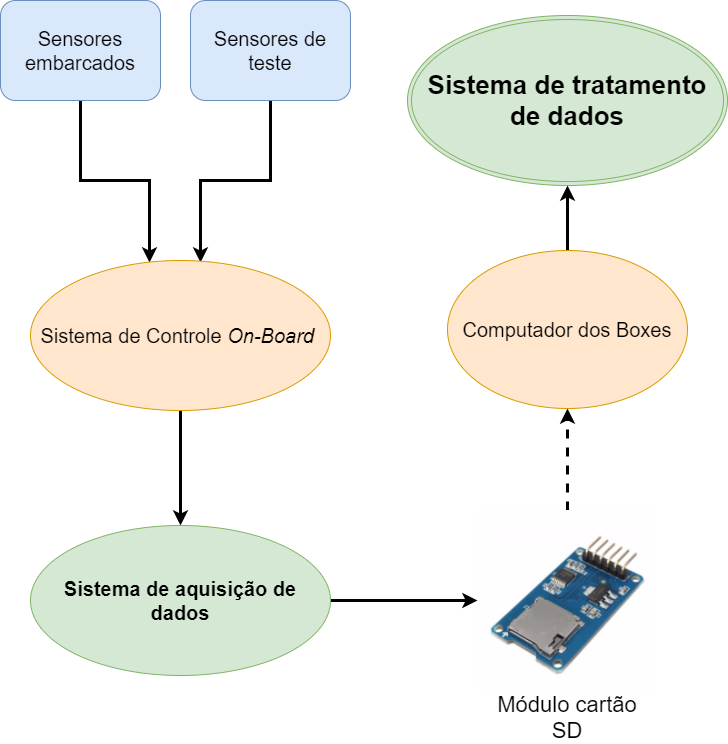
\includegraphics[scale=0.3]{geral.png} 
		\caption*{Fonte: Autor.}
		\label{fig:geral}
\end{figure} 


\subsection{Objetivos Específicos} 

\begin{itemize}[label={-}]
	\item O sistema deve ser independente em relação ao meio em que os dados são transportados do SCOB para os boxes; Desta forma em atualizações futuras o método atual de transferência de dados pode ser substituido por telemetria;
	\item O \textit{software} deve ser independente de sistema operacional;
	\item O \textit{software} deve possuir informações específicas para cada área da engenharia automobilística;
	\item O \textit{software} deve ser construido de forma a facilitar a manutenção evolutiva, preparado para chegada de novos sensores;
	\item Deve ser criada e atualizada uma documentação do \textit{software};
	\item Deve se instaurar uma cultura de utilização de engenharia de \textit{software} para facilitar manutenções adaptativas e manutenções corretivas.
\end{itemize}
